\section{Testing Phase of Machine Learning Model with Test Dataset} \label{Section: Testing Phase of ML Model}
\subsection{Data Throughput Strength Classifier}
The trained machine learning model (classifier) is evaluated with the test set which contains 10\% of the data set. The performance of the data throughput strength classifier is illustrated in a confusion matrix by making use of the heatmap function available. The vertical columns represent the predicted class while the horizontal rows represent the actual class of the data points. A classification report is also produced to evaluate the performance of the classifier which displays measurement metrics such as accuracy, recall, precision, and F1-score. 

\subsubsection{k-NN Algorithm with 800 Data Points}
Firstly, the model built with the k-Nearest Neighbour algorithm using the 800 data points is first tested. The confusion matrix for the model is shown in Fig. \ref{fig_cm1}.The diagonal values in the matrix represent the correctly classified data points with respect to their classes. Data points outside of the diagonal values are misclassified points. For example, there are four points from the `Strong' data throughput class misclassified under the `Moderate' data throughput class. One data point from the `Moderate' class was misclassified as the `Weak' class. Next, three data points from the `Very Strong' class were misclassified as the 'Strong' class.

\begin{figure} [ht]
    \centering
    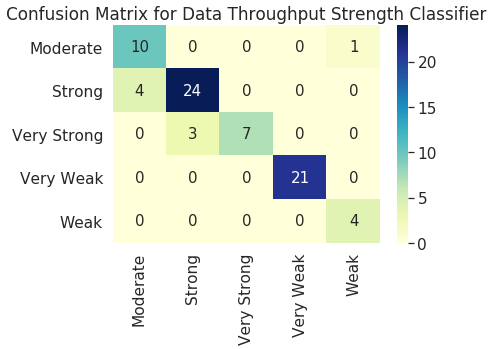
\includegraphics[scale=1.0]{pages/Chapter5/Chapter 5 images/knn_800.PNG}
    \caption{Confusion matrix of Data Throughput Strength Classifier}
    \label{fig_cm1}
\end{figure}

A classification report for the tested model is shown in Figure \ref{fig_crknn}. The precision, recall and F1-score for each class is also displayed. The support column shows the actual amount of data points that belong to their corresponding classes. The `macro avg' represents the average precision, recall and F1-score across the five classes. The `weighted avg' shows the average of the three metrics where the metric of each class is multiplied by a weight during the calculation of the average values. This step is done to give a better average value when there are imbalance data points across the five classes of data.  

The accuracy achieved by the model is 89.2\%. The weighted average values of precision, recall and F1-score obtained are 90.5\%, 89.2\% and 89.2\% which is fairly good.  

\begin{figure} [ht]
    \centering
    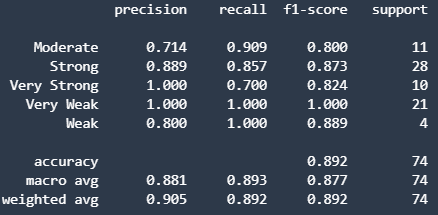
\includegraphics[scale=1.3]{pages/Chapter5/Chapter 5 images/C_report_knn.PNG}
    \caption{Classification report of the k-NN classifier}
    \label{fig_crknn}
\end{figure}


\subsubsection{k-NN Algorithm with 6000 Data Points}
The confusion matrix is produced for the trained model with the 6000 data points and can be shown in  Fig. \ref{fig_cm1}. Five data points from the `Very Strong' class were misclassified as the `Strong' class while three data points from the `Weak' class were misclassified as the `Very Weak' class. One point from the `Moderate' class were misclassified as the `Weak' class.

\begin{figure} [ht]
    \centering
    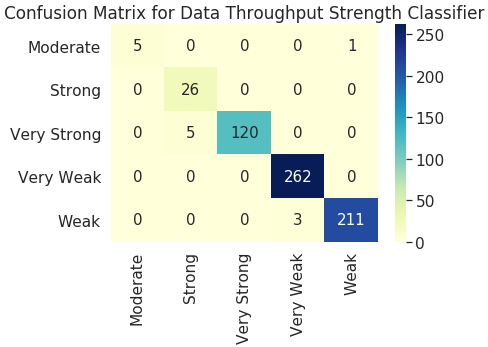
\includegraphics[scale=1.0]{pages/Chapter5/Chapter 5 images/knn_6k.PNG}
    \caption{Confusion matrix of Data Throughput Strength Classifier}
    \label{fig_cm1}
\end{figure}

The classification report for the tested model is obtained. The accuracy achieved by the model is approximately 98.6\%. The weighted average precision, recall and F1-score obtained are 98.7\%, 98.6\% and 98.6\% respectively. This model has a better performance than the previous model. Therefore, the model with a larger data set gives a better overall performance in classifying data.


\begin{figure} [ht]
    \centering
    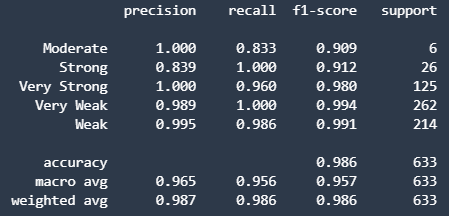
\includegraphics[scale=1.3]{pages/Chapter5/Chapter 5 images/C_report_knn6k.PNG}
    \caption{Classification report of the k-NN classifier}
    \label{fig_crknn}
\end{figure}

\subsubsection{XGBoost Algorithm with 800 Data Points}
Since the classifier achieved a very low accuracy during its training and validation phase, it will not be used to predict the test data.
% \begin{figure} [ht]
%     \centering
%     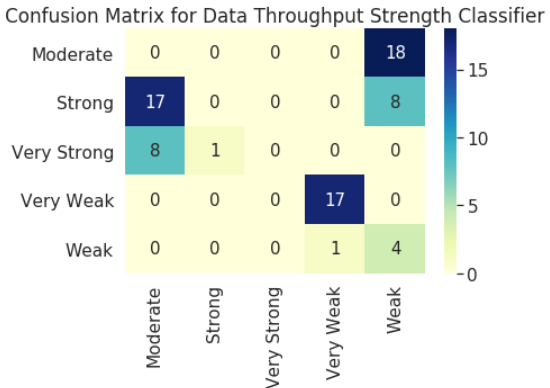
\includegraphics[scale=1.0]{pages/Chapter5/Chapter 5 images/cm_xgb800.PNG}
%     \caption{Confusion matrix of the XGBoost classifier}
%     \label{fig_cmxgb}
% \end{figure}

% \begin{figure} [ht]
%     \centering
%     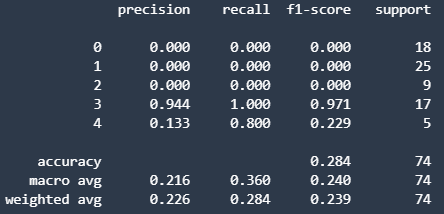
\includegraphics[scale=1.3]{pages/Chapter5/Chapter 5 images/c_report_xgb.PNG}
%     \caption{Classification report of the XGB classifier}
%     \label{fig_crxgb}
% \end{figure}
\subsubsection{XGBoost Algorithm with 6000 Data Points}
The variable defined for the deployed trained model is used to predict the test dataset. The confusion matrix for the data throughput classifier is then obtained and shown in Fig. \ref{fig_cmxgb}. It can be seen that four data points that actually belong to the `Very Strong' class were misclassified as the 'Strong' class. Four data points from the `Strong' class were misclassified as the `Very Strong' class. Two data points from the `Weak' class were misclassified as the `Very Weak' class.

\begin{figure} [ht]
    \centering
    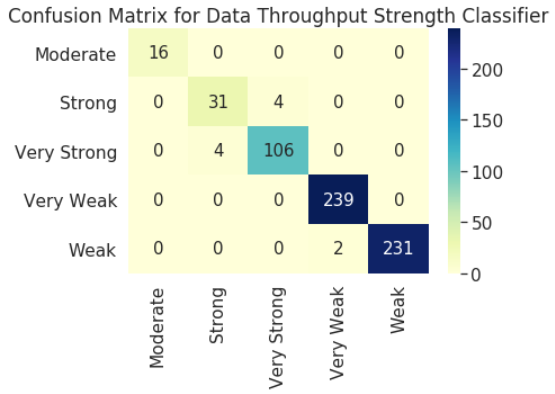
\includegraphics[scale=1.0]{pages/Chapter5/Chapter 5 images/cm_xgb6k.PNG}
    \caption{Confusion matrix of the XGBoost classifier}
    \label{fig_cmxgb}
\end{figure}

 The classification report for the tested model is also produced and shown in Fig. \ref{fig_crxgb}. The accuracy achieved by the final model is 98.4\%. The weighted average precision, recall and F1-score obtained are 98.4\%. 98.4\% and 98.4\% respectively. Thus, it has  a good overall performance. 
 
\begin{figure} [ht]
    \centering
    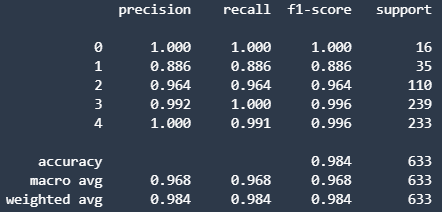
\includegraphics[scale=1.3]{pages/Chapter5/Chapter 5 images/C_report_xgb6k.PNG}
    \caption{Classification report of the XGBoost classifier}
    \label{fig_crxgb}
\end{figure}
\section{Testing Phase of Machine Learning Model with Postman}
\label{post_man_testing}
After testing the performance of the classifier with the test dataset, the XGBoost model with an accuracy of 98.4\% is used to predict new test data. The endpoint of the model, ``sagemaker-xgboost-2020-12-22-20-52-53-943'' is included in the environmental variable of the Lambda function created. The new test data is classified with the deployed endpoint using Postman, which is an HTTP client for testing web services. The invoke URL is obtained during the API Gateway deployment and is placed onto the Postman client as shown in Fig. \ref{fig_post}. The new test data is also put into the `body' section followed by executing the `send' button. The test data passes through an event where the Lambda function filters out specified parameters needed for the classification process.
\begin{figure} [ht]
    \centering
    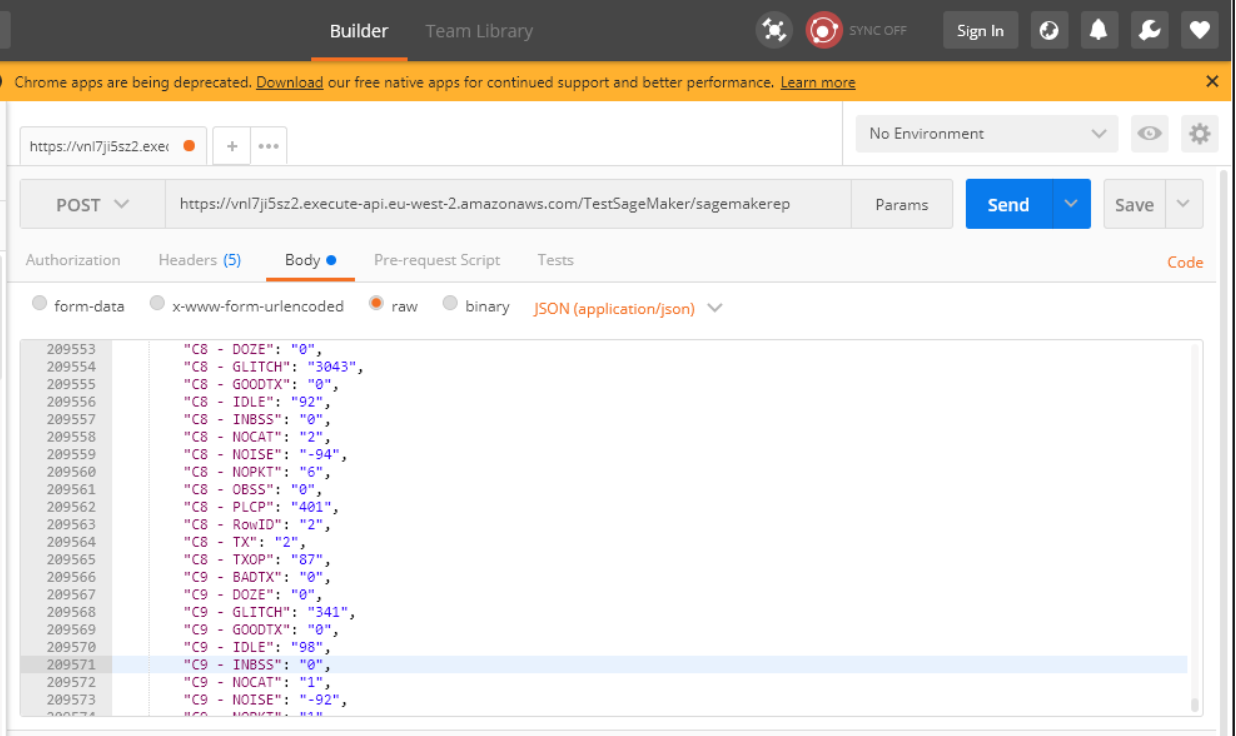
\includegraphics[scale=0.55]{pages/Chapter5/Chapter 5 images/POSTMAN1.PNG}
    \caption{Classification of new test data in Postman}
    \label{fig_post}
\end{figure}

 The results of the classification are then displayed below in the `body' section as shown in Fig. \ref{fig_postr}. The classification results are displayed in an array of numeric values where each value represents the class of each data point. Each numeric value represents the data throughput strength of the corresponding data point. For example, the first value of `3.0' in the array represents the first data point which belongs to the `Very Weak' class.
 
 \begin{figure} [ht]
    \centering
    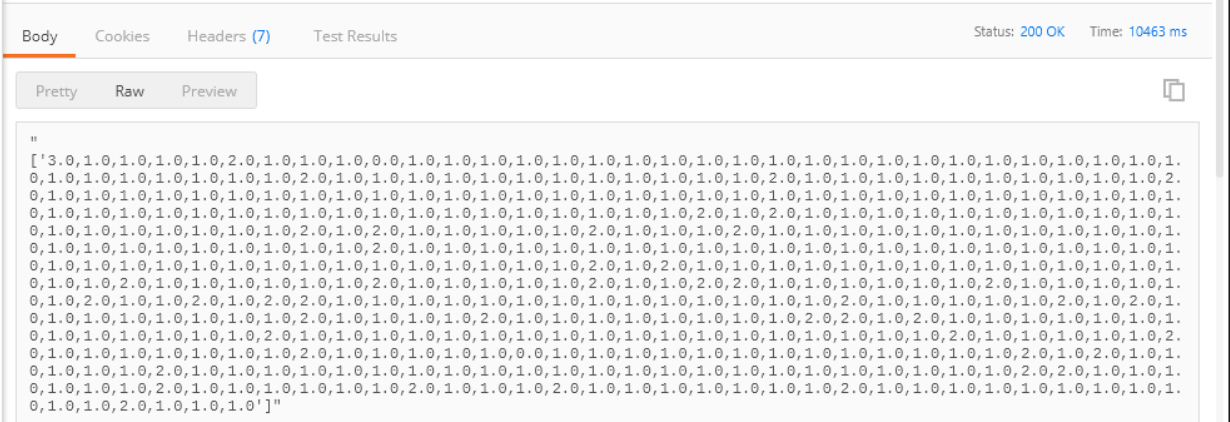
\includegraphics[scale=0.56]{pages/Chapter5/Chapter 5 images/PostmanR.PNG}
    \caption{Classification Results of each Data Point in Postman}
    \label{fig_postr}
\end{figure}